% GNUPLOT: LaTeX picture with Postscript
\documentclass{minimal}
% Set font size
\makeatletter
\def\@ptsize{1}
\InputIfFileExists{size11.clo}{}{%
   \GenericError{(gnuplot) \space\space\space\@spaces}{%
      Gnuplot Error: File `size11.clo' not found! Could not set font size%
   }{See the gnuplot documentation for explanation.%
   }{For using a font size a file `size<fontsize>.clo' has to exist.
        Falling back ^^Jto default fontsize 10pt.}%
  \def\@ptsize{0}
  \input{size10.clo}%
}%
\makeatother
% Load packages
\usepackage{calc}
\usepackage{graphicx}
\usepackage{color}
\makeatletter
% Select an appropriate default driver (from TeXLive graphics.cfg)
\begingroup
  \chardef\x=0 %
  % check pdfTeX
  \@ifundefined{pdfoutput}{}{%
    \ifcase\pdfoutput
    \else
      \chardef\x=1 %
    \fi
  }%
  % check VTeX
  \@ifundefined{OpMode}{}{%
    \chardef\x=2 %
  }%
\expandafter\endgroup
\ifcase\x
  % default case
  \PassOptionsToPackage{dvips}{geometry}
\or
  % pdfTeX is running in pdf mode
  \PassOptionsToPackage{pdftex}{geometry}
\else
  % VTeX is running
  \PassOptionsToPackage{vtex}{geometry}
\fi
\makeatother
% Set papersize
\usepackage[papersize={1008.00bp,288.00bp},text={1008.00bp,288.00bp}]{geometry}
% No page numbers and no paragraph indentation
\pagestyle{empty}
\setlength{\parindent}{0bp}%
% Load configuration file
\InputIfFileExists{gnuplot.cfg}{%
  \typeout{Using configuration file gnuplot.cfg}%
}{%
 \typeout{No configuration file gnuplot.cfg found.}%
}%
%
\begin{document}
\begingroup
  \makeatletter
  \providecommand\color[2][]{%
    \GenericError{(gnuplot) \space\space\space\@spaces}{%
      Package color not loaded in conjunction with
      terminal option `colourtext'%
    }{See the gnuplot documentation for explanation.%
    }{Either use 'blacktext' in gnuplot or load the package
      color.sty in LaTeX.}%
    \renewcommand\color[2][]{}%
  }%
  \providecommand\includegraphics[2][]{%
    \GenericError{(gnuplot) \space\space\space\@spaces}{%
      Package graphicx or graphics not loaded%
    }{See the gnuplot documentation for explanation.%
    }{The gnuplot epslatex terminal needs graphicx.sty or graphics.sty.}%
    \renewcommand\includegraphics[2][]{}%
  }%
  \providecommand\rotatebox[2]{#2}%
  \@ifundefined{ifGPcolor}{%
    \newif\ifGPcolor
    \GPcolortrue
  }{}%
  \@ifundefined{ifGPblacktext}{%
    \newif\ifGPblacktext
    \GPblacktexttrue
  }{}%
  % define a \g@addto@macro without @ in the name:
  \let\gplgaddtomacro\g@addto@macro
  % define empty templates for all commands taking text:
  \gdef\gplbacktext{}%
  \gdef\gplfronttext{}%
  \makeatother
  \ifGPblacktext
    % no textcolor at all
    \def\colorrgb#1{}%
    \def\colorgray#1{}%
  \else
    % gray or color?
    \ifGPcolor
      \def\colorrgb#1{\color[rgb]{#1}}%
      \def\colorgray#1{\color[gray]{#1}}%
      \expandafter\def\csname LTw\endcsname{\color{white}}%
      \expandafter\def\csname LTb\endcsname{\color{black}}%
      \expandafter\def\csname LTa\endcsname{\color{black}}%
      \expandafter\def\csname LT0\endcsname{\color[rgb]{1,0,0}}%
      \expandafter\def\csname LT1\endcsname{\color[rgb]{0,1,0}}%
      \expandafter\def\csname LT2\endcsname{\color[rgb]{0,0,1}}%
      \expandafter\def\csname LT3\endcsname{\color[rgb]{1,0,1}}%
      \expandafter\def\csname LT4\endcsname{\color[rgb]{0,1,1}}%
      \expandafter\def\csname LT5\endcsname{\color[rgb]{1,1,0}}%
      \expandafter\def\csname LT6\endcsname{\color[rgb]{0,0,0}}%
      \expandafter\def\csname LT7\endcsname{\color[rgb]{1,0.3,0}}%
      \expandafter\def\csname LT8\endcsname{\color[rgb]{0.5,0.5,0.5}}%
    \else
      % gray
      \def\colorrgb#1{\color{black}}%
      \def\colorgray#1{\color[gray]{#1}}%
      \expandafter\def\csname LTw\endcsname{\color{white}}%
      \expandafter\def\csname LTb\endcsname{\color{black}}%
      \expandafter\def\csname LTa\endcsname{\color{black}}%
      \expandafter\def\csname LT0\endcsname{\color{black}}%
      \expandafter\def\csname LT1\endcsname{\color{black}}%
      \expandafter\def\csname LT2\endcsname{\color{black}}%
      \expandafter\def\csname LT3\endcsname{\color{black}}%
      \expandafter\def\csname LT4\endcsname{\color{black}}%
      \expandafter\def\csname LT5\endcsname{\color{black}}%
      \expandafter\def\csname LT6\endcsname{\color{black}}%
      \expandafter\def\csname LT7\endcsname{\color{black}}%
      \expandafter\def\csname LT8\endcsname{\color{black}}%
    \fi
  \fi
    \setlength{\unitlength}{0.0500bp}%
    \ifx\gptboxheight\undefined%
      \newlength{\gptboxheight}%
      \newlength{\gptboxwidth}%
      \newsavebox{\gptboxtext}%
    \fi%
    \setlength{\fboxrule}{0.5pt}%
    \setlength{\fboxsep}{1pt}%
    \definecolor{tbcol}{rgb}{1,1,1}%
\begin{picture}(20160.00,5760.00)%
    \gplgaddtomacro\gplbacktext{%
      \csname LTb\endcsname%%
      \put(1188,880){\makebox(0,0)[r]{\strut{}\Large$10^{-7}$}}%
      \put(1188,1514){\makebox(0,0)[r]{\strut{}\Large$10^{-6}$}}%
      \put(1188,2148){\makebox(0,0)[r]{\strut{}\Large$10^{-5}$}}%
      \put(1188,2782){\makebox(0,0)[r]{\strut{}\Large$10^{-4}$}}%
      \put(1188,3417){\makebox(0,0)[r]{\strut{}\Large$10^{-3}$}}%
      \put(1188,4051){\makebox(0,0)[r]{\strut{}\Large$10^{-2}$}}%
      \put(1188,4685){\makebox(0,0)[r]{\strut{}\Large$10^{-1}$}}%
      \put(1188,5319){\makebox(0,0)[r]{\strut{}\Large$10^{0}$}}%
      \put(1320,660){\makebox(0,0){\strut{}\Large$1$}}%
      \put(3574,660){\makebox(0,0){\strut{}\Large$10$}}%
      \put(5827,660){\makebox(0,0){\strut{}\Large$100$}}%
      \put(8081,660){\makebox(0,0){\strut{}\Large$1000$}}%
      \put(1692,4209){\makebox(0,0)[l]{\strut{}\huge$\alpha=1.1$}}%
      \put(2064,5408){\makebox(0,0)[l]{\strut{}\huge (a)}}%
      \put(2659,5408){\makebox(0,0)[l]{\strut{}\huge Trans. Ising}}%
      \put(6155,4875){\makebox(0,0)[l]{\strut{}\huge$n^{-0.2}$}}%
      \put(4296,3455){\makebox(0,0)[l]{\strut{}\LARGE$n^{-0.2}$}}%
    }%
    \gplgaddtomacro\gplfronttext{%
      \csname LTb\endcsname%%
      \put(9315,5559){\makebox(0,0)[r]{\strut{}\Large$N=256$}}%
      \csname LTb\endcsname%%
      \put(9315,5239){\makebox(0,0)[r]{\strut{}\Large$N=512$}}%
      \csname LTb\endcsname%%
      \put(9315,4919){\makebox(0,0)[r]{\strut{}\Large$N=1024$}}%
      \csname LTb\endcsname%%
      \put(9315,4599){\makebox(0,0)[r]{\strut{}\Large$N=2048$}}%
      \csname LTb\endcsname%%
      \put(9315,4279){\makebox(0,0)[r]{\strut{}\Large$N=4096$}}%
      \csname LTb\endcsname%%
      \put(319,3099){\rotatebox{-270.00}{\makebox(0,0){\strut{}\Huge$\langle \mathcal{J}_n \mathcal{J}_0 \rangle$}}}%
      \put(5039,330){\makebox(0,0){\strut{}\Huge$n$}}%
    }%
    \gplgaddtomacro\gplbacktext{%
      \csname LTb\endcsname%%
      \put(2690,1440){\makebox(0,0)[r]{\strut{}$10^{-7}$}}%
      \put(2690,2055){\makebox(0,0)[r]{\strut{}$10^{-5}$}}%
      \put(2690,2669){\makebox(0,0)[r]{\strut{}$10^{-3}$}}%
      \put(2690,3284){\makebox(0,0)[r]{\strut{}$10^{-1}$}}%
      \put(3148,1220){\makebox(0,0){\strut{}$10$}}%
      \put(4233,1220){\makebox(0,0){\strut{}$100$}}%
      \put(5318,1220){\makebox(0,0){\strut{}$1000$}}%
    }%
    \gplgaddtomacro\gplfronttext{%
      \csname LTb\endcsname%%
      \put(1755,2515){\rotatebox{-270.00}{\makebox(0,0){\strut{}\LARGE$\displaystyle\int^{\infty}_0 dt \langle \mathcal{J}_n(t) \mathcal{J}_0 \rangle$}}}%
      \put(5949,1440){\makebox(0,0){\strut{}\LARGE$n$}}%
    }%
    \gplgaddtomacro\gplbacktext{%
      \csname LTb\endcsname%%
      \put(11268,1435){\makebox(0,0)[r]{\strut{}\Large$10^{-8}$}}%
      \put(11268,1990){\makebox(0,0)[r]{\strut{}\Large$10^{-7}$}}%
      \put(11268,2545){\makebox(0,0)[r]{\strut{}\Large$10^{-6}$}}%
      \put(11268,3100){\makebox(0,0)[r]{\strut{}\Large$10^{-5}$}}%
      \put(11268,3654){\makebox(0,0)[r]{\strut{}\Large$10^{-4}$}}%
      \put(11268,4209){\makebox(0,0)[r]{\strut{}\Large$10^{-3}$}}%
      \put(11268,4764){\makebox(0,0)[r]{\strut{}\Large$10^{-2}$}}%
      \put(11268,5319){\makebox(0,0)[r]{\strut{}\Large$10^{-1}$}}%
      \put(11400,660){\makebox(0,0){\strut{}\Large$1$}}%
      \put(13654,660){\makebox(0,0){\strut{}\Large$10$}}%
      \put(15907,660){\makebox(0,0){\strut{}\Large$100$}}%
      \put(18161,660){\makebox(0,0){\strut{}\Large$1000$}}%
      \put(11772,4209){\makebox(0,0)[l]{\strut{}\huge$\alpha=1.6$}}%
      \put(12144,5408){\makebox(0,0)[l]{\strut{}\huge(b)}}%
      \put(12739,5408){\makebox(0,0)[l]{\strut{}\huge Trans. Ising}}%
      \put(16235,3899){\makebox(0,0)[l]{\strut{}\huge$n^{-1.2}$}}%
      \put(14524,2922){\makebox(0,0)[l]{\strut{}\LARGE$n^{-1.2}$}}%
    }%
    \gplgaddtomacro\gplfronttext{%
      \csname LTb\endcsname%%
      \put(18577,5559){\makebox(0,0)[r]{\strut{}\Large$N=256$}}%
      \csname LTb\endcsname%%
      \put(18577,5239){\makebox(0,0)[r]{\strut{}\Large$N=512$}}%
      \csname LTb\endcsname%%
      \put(18577,4919){\makebox(0,0)[r]{\strut{}\Large$N=1024$}}%
      \csname LTb\endcsname%%
      \put(18577,4599){\makebox(0,0)[r]{\strut{}\Large$N=2048$}}%
      \csname LTb\endcsname%%
      \put(18577,4279){\makebox(0,0)[r]{\strut{}\Large$N=4096$}}%
      \csname LTb\endcsname%%
      \put(10399,3099){\rotatebox{-270.00}{\makebox(0,0){\strut{}\Huge$\langle \mathcal{J}_n \mathcal{J}_0 \rangle$}}}%
      \put(15119,330){\makebox(0,0){\strut{}\Huge$n$}}%
    }%
    \gplgaddtomacro\gplbacktext{%
      \csname LTb\endcsname%%
      \put(12770,1440){\makebox(0,0)[r]{\strut{}$10^{-7}$}}%
      \put(12770,2157){\makebox(0,0)[r]{\strut{}$10^{-5}$}}%
      \put(12770,2874){\makebox(0,0)[r]{\strut{}$10^{-3}$}}%
      \put(12770,3591){\makebox(0,0)[r]{\strut{}$10^{-1}$}}%
      \put(13228,1220){\makebox(0,0){\strut{}$10$}}%
      \put(14313,1220){\makebox(0,0){\strut{}$100$}}%
      \put(15398,1220){\makebox(0,0){\strut{}$1000$}}%
    }%
    \gplgaddtomacro\gplfronttext{%
      \csname LTb\endcsname%%
      \put(11835,2515){\rotatebox{-270.00}{\makebox(0,0){\strut{}\LARGE$\displaystyle\int^{\infty}_0 dt \langle \mathcal{J}_n(t) \mathcal{J}_0 \rangle$}}}%
      \put(16029,1440){\makebox(0,0){\strut{}\LARGE$n$}}%
    }%
    \gplbacktext
    \put(0,0){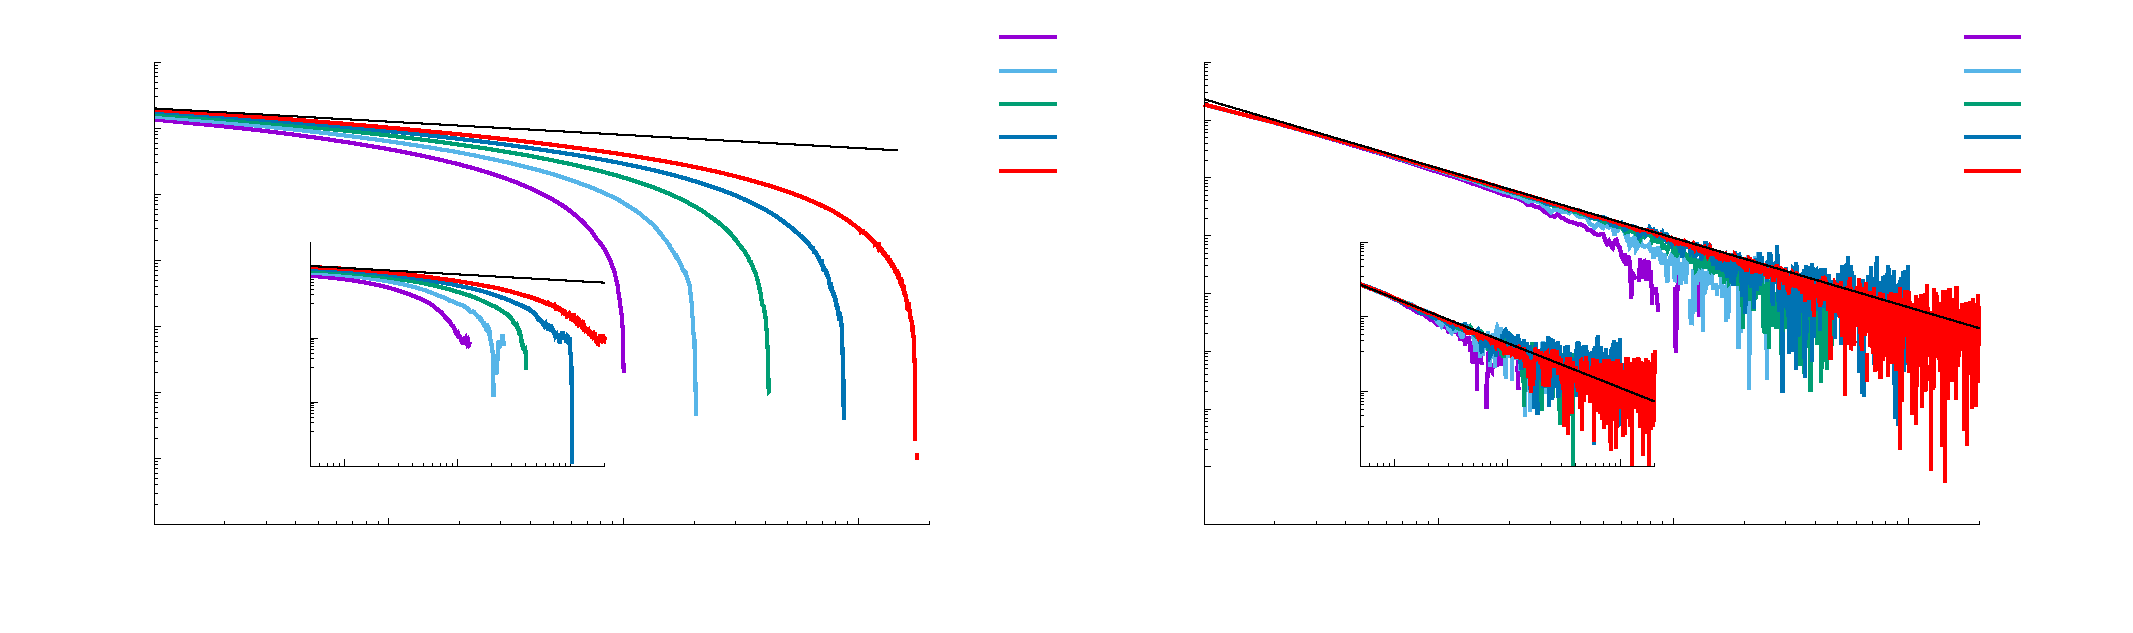
\includegraphics[width={1008.00bp},height={288.00bp}]{fig2_sup2-inc}}%
    \gplfronttext
  \end{picture}%
\endgroup
\end{document}
